\documentclass{article}


\usepackage{arxiv}

\usepackage[utf8]{inputenc} % allow utf-8 input
\usepackage[T1]{fontenc}    % use 8-bit T1 fonts
\usepackage{hyperref}       % hyperlinks
\usepackage{url}            % simple URL typesetting
\usepackage{booktabs}       % professional-quality tables
\usepackage{amsfonts}       % blackboard math symbols
\usepackage{nicefrac}       % compact symbols for 1/2, etc.
\usepackage{microtype}      % microtypography
\usepackage{graphicx}
\usepackage{epstopdf, epsfig}
\usepackage{subfigure}
\usepackage{pgfplotstable}
\usepackage{booktabs}
\usepackage{filecontents}
\usepackage{longtable}
\usepackage{array}
\usepackage{amsmath} % for \boldsymbol macro
\usepackage{bm}
\usepackage{amsmath}%
\usepackage{MnSymbol}%
\usepackage{wasysym}%

\title{The title}
\rhead{\scshape Short title \today}

\author{
  Whoami\\
  affiliation\\
  \texttt{email} \\
   \And
  Whoami\\
  affiliation\\
  \texttt{email} \\
}

\begin{document}
\maketitle

\begin{abstract}
  The abstract
\end{abstract}

\keywords{Keyword 1 \and Keyword 2}

\section{Some section}

Blabla.

\subsection{some subsection}

Blabla, and Fig. \ref{fig:fig_handle}, and previous work directly within the text from \citet{JGRC21649}, also can be shown in parenthesis \citep{JGRC21649}.

Some more old blabla that should be removed.

\begin{figure}[h]
  \begin{center}
    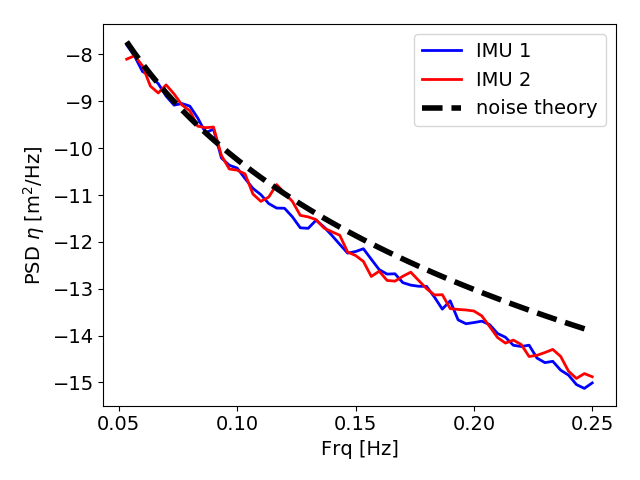
\includegraphics[width=.45\textwidth]{./Figures/noise_verification}
    \caption{\label{fig:fig_handle} Some caption.}
  \end{center}
\end{figure}

Also some equations Eq. (\ref{eq:eq_handle}):

\begin{equation}
	\eta(t) = \mathrm{IFFT}\left[H(f)\mathrm{FFT}(a_z)\right],
	\label{eq:eq_handle}
\end{equation}

where $\mathrm{FFT}$ and $\mathrm{IFFT}$ denote the Fourier and Inverse Fourier transforms respectively and $H(f)$ is the half-cosine taper function. \\

And some table, Tab. \ref{tab:tab_handle}.

\begin{table}[h]
\begin{center}
	\begin{tabular}{c|c}
	Variable & Machine precision \\ \hline
		Significant wave height (from time series) & 32-bit floating point \\
		$R(f)$ at 25 frequencies & 25 $\times$ 16-bit signed integer 
	\end{tabular}
	\end{center}
	\caption{Some label.}
	\label{tab:tab_handle}
\end{table}

\section{Conclusion and future work}

We shall conclude! ...

\section*{Acknowledgement}

... And acknowledge

\section*{Appendix A: something extra long}

An Appendix never hurt.

\bibliographystyle{jfm}
\bibliography{bibliography}


\end{document}
